\documentclass[final]{hcmuitthesis}
\usepackage[utf8]{vietnam}
\usepackage{placeins}
\usepackage{amsfonts}
\usepackage{textcomp}
\usepackage{dblfloatfix}
\usepackage{lineno}
\usepackage{amssymb}
\usepackage{tabularx,booktabs}
\usepackage{longtable, lipsum}
\usepackage{amsmath}
\usepackage{mathtools}
\usepackage{graphicx}
\usepackage{lscape}
\usepackage{caption}
\usepackage{hyperref}
\usepackage[sorting=nyt]{biblatex}
\usepackage{mathtools}
\usepackage{lipsum}
\usepackage{fancyhdr}
\usepackage{titlesec}
\usepackage{makecell}
\usepackage{listings}
\usepackage{subcaption}
\usepackage{adjustbox}
\usepackage[vietnamese,english]{babel}

% Config reference source file
\addbibresource{references/chapter2.bib}

% Config figure path
\graphicspath{ {./graphics} }

% Config for math in quantum computin
\DeclarePairedDelimiter\bra{\langle}{\rvert}
\DeclarePairedDelimiter\ket{\lvert}{\rangle}
\DeclarePairedDelimiterX\braket[2]{\langle}{\rangle}{#1 \delimsize\vert#2}

% Config listings 
\lstset{
  frame=tb,
  aboveskip=3mm,
  belowskip=3mm,
  showstringspaces=false,
  columns=fullflexible,
  basicstyle={\small\ttfamily},
  numbers=left,
  numberstyle=\tiny\color{gray},
  keywordstyle=\color{blue},
  commentstyle=\color{dkgreen},
  stringstyle=\color{mauve},
  breaklines=true,
  postbreak=\mbox{\textcolor{red}{$\hookrightarrow$}\space},
  tabsize=3
}

% Config information thesis
% =========== Thay đổi thông tin tại phần này ===========
\upperuniname{ĐẠI HỌC QUỐC GIA THÀNH PHỐ HỒ CHÍ MINH}
\uniname{TRƯỜNG ĐẠI HỌC CÔNG NGHỆ THÔNG TIN}
\deptname{KHOA MẠNG MÁY TÍNH VÀ TRUYỀN THÔNG}
\stumajor{KỸ SƯ NGÀNH AN TOÀN THÔNG TIN}
\title{SỬ DỤNG LATEX TRONG SOẠN THẢO KHÓA LUẬN TỐT NGHIỆP}
\titleen{USING LATEX IN WRITING GRADUATION THESIS}
\supervisor{GIẢNG VIÊN HƯỚNG DẪN}
\supervisorname{TS. GOOGLE}
\stuname{NGUYỄN HỒNG SƠN }
\stunamewithid{NGUYỄN HỒNG SƠN - 17520988}
\reporttime{NĂM 2024}
\reporttype{KHÓA LUẬN TỐT NGHIỆP}
\instruction{GIẢNG VIÊN HƯỚNG DẪN}
\reportplace{TP. HỒ CHÍ MINH}
% =========== Hết phần thay đổi thông tin ===========

% Begin thesis
\begin{document}

\coverpage%
\secondcoverpage%

% Begin above main thesis
\frontmatter
\chapter*{\centering\Large{Thông tin hội đồng chấm khóa luận tốt nghiệp}}
\addcontentsline{toc}{chapter}{Thông tin hội đồng chấm khóa luận tốt nghiệp}
Hội đồng chấm khóa luận tốt nghiệp, thành lập theo Quyết định số 463/QĐĐHCNTT ngày 23 tháng 7 năm 2021 của Hiệu trưởng Trường Đại học Công nghệ
Thông tin.
\begin{center}
    \begin{tabular}{ p{.4\textwidth} p{.3\textwidth}} 
        1. TS. Nguyễn Tuấn Nam  & Chủ tịch \\
        2. ThS. Nguyễn Duy   & Ủy viên \\ 
        3. ThS. Trần Hồng Nghi & Thư ký \\ 
    \end{tabular} 
\end{center}



\chapter*{\centering\Large{Lời cảm ơn}}
\addcontentsline{toc}{chapter}{Lời cảm ơn}
Không ai đạt được điều gì đó to lớn mà không nhờ sự giúp đỡ của những
người xung quanh, cho dù là trực tiếp hay gián tiếp đi nữa. Để hoàn thành được
khóa luận này, nhóm tác giả may mắn nhận được nhiều sự giúp đỡ và hỗ trợ từ
quý thầy, cô, anh chị, bạn bè và người thân. Nhóm tác giả xin dành những trang
đầu tiên này để bày tỏ lòng tri ân của mình tới tất cả mọi người, những người đã
đồng hành cùng nhóm trong khoảng thời gian vừa qua. \\
\indent Đầu tiên, nhóm tác giả xin gửi lời cảm ơn sâu sắc đến toàn thể các thầy cô
của Trường Đại học Công nghệ Thông tin nói chung và các thầy cô khoa Mạng
máy tính và Truyền thông nói riêng. Nhờ những kiến thức quý giá mà thầy cô đã
truyền đạt, cũng như việc hỗ trợ tận tình trong suốt khoảng thời gian thực hiện,
nhóm đã hoàn thành khóa luận và đạt được các kết quả đáng ghi nhận.
Nhóm tác giả xin đặc biệt cảm ơn TS. Nguyễn Ngọc Tự là người đã truyền
cảm hứng, tận tình hướng dẫn và hỗ trợ tận tình về kiến thức, tạo môi trường thuận
lợi để nhóm có thể học hỏi, trao đổi với các bạn, các em trong nhóm nghiên cứu.
Đây là những kiến thức, kinh nghiệm quý giá, không chỉ có tác dụng trong khóa
luận tốt nghiệp này mà còn trong khoảng thời gian làm việc trong chặng đường
tiếp theo. \\
\indent Trong giai đoạn dịch bệnh khó khăn, tình hình ngày càng phức tạp, dù có
khó khăn trong nhiều công việc, nhóm nhận được nhiều sự giúp đỡ và động viên
từ thầy cô và bạn bè. Đây là động lực to lớn thúc đẩy nhóm làm việc trong suốt
quá trình tìm hiểu và hoàn thành khóa luận này. \\
\indent Cuối cùng, nhóm tác giả không quên bày tỏ lòng tri ân đến gia đình và người
thân, những người đã luôn là những hậu phương vững chắc và luôn ủng hộ từng
quyết định mà nhóm đưa ra. \\
\indent Mặc dù đã nỗ lực rất nhiều để luận văn được hoàn thiện nhất, song khó có
thể tránh khỏi thiếu sót và hạn chế. Kính mong nhận được sự thông cảm và ý kiến
đóng góp từ quý thầy cô và các bạn.\\

\begin{flushright}
\textit {TP. Hồ Chí Minh, ngày 12 tháng 7 năm 2021} \\
\textit {Nhóm tác giả}
\end{flushright}


\tableofcontents
\clearpage
\listoffigures
\clearpage
\listoftables
\clearpage
\lstlistoflistings
\chapter*{\centering\Large{Danh sách từ viết tắt}}
\addcontentsline{toc}{chapter}{Danh sách từ viết tắt}
\begin{tabular}{| p{.4\textwidth} |p{.4\textwidth} |}
\hline
        KLTN &  Khóa luận tốt nghiệp\\
        \hline
        GVHD & Giảng viên hướng dẫn \\
        \hline
\end{tabular} \\



\chapter*{\centering\Large{Danh mục từ tạm dịch}}
\addcontentsline{toc}{chapter}{Danh mục từ tạm dịch}
\begin{tabular}{| p{.4\textwidth} |p{.4\textwidth} |}
\hline
        Machine Learning &  Học máy\\
        \hline
        Deep Learning & Học sâu \\
        \hline
        Reinforcement learning & Học tăng cường \\
        \hline
        Federated Learning & Học liên kết\\
        \hline
\end{tabular} \\



\clearpage

% Begin main thesis, start page numbering
\counterwithin{equation}{chapter}
\counterwithin{table}{chapter}
\counterwithin{figure}{chapter}
\setcounter{secnumdepth}{3}
\mainmatter

% Config page header
\fancyhf{}
\fancyfoot[C]{\thepage}
% \chapter*{Tóm tắt khóa luận}
\chapter*{\centering\Large{Tóm tắt khóa luận}}
\addcontentsline{toc}{chapter}{Tóm tắt khóa luận}

Vào năm 2021, dù cảm thấy không có đủ năng lực để theo tiếp đồ án chuyên ngành, mình thực hiện khóa luận do chương trình đào tạo cũ bắt buộc làm luận văn. Nhóm mình hai người, thực hiện tìm hiểu và viết luận văn trong khoảng thời gian dịch bệnh đầy khó khăn.

Làm xong rồi, nhưng việc báo cáo nó cũng không phải dễ. Mỗi người một nơi, cùng làm việc trên Word khó khăn do định dạng không đồng bộ, chèn hình và bảng làm xáo trộn các trang, đánh số bảng biểu, hình ảnh, tiêu đề dễ bị sai sót. Khó khăn nhất là việc viết và đánh số tài liệu tham khảo.

Sau này, khi học thạc sĩ và làm việc trên linux, một mặt cần tính chuyên nghiệp cao trong viết báo cáo, mặt khác sử dụng Word online trên linux rất bất tiện, mình đã làm quen và dần dần chuyển hẳn việc viết báo cáo trên latex, kể cả các báo cáo ở công ty.

Nhằm lưu lại các cú pháp mình sử dụng, đồng thời giúp các bạn sinh viên viết khóa luận dễ dàng hơn, mình đã thiết kế và viết báo cáo này. Các bạn sinh viên UIT nói riêng và người dùng khác nói chung có thể tùy ý sử dụng, thay đổi dự án này tùy theo nhu cầu.

Phần còn lại của luận văn có cấu trúc như sau
\begin{itemize}
    \item Chương \ref{chap:chap1-introduce} giới thiệu khái quát chung về cấu trúc thư mục trong dự án, các cài đặt, cấu hình cần thay đổi khi sử dụng.
    \item Chương \ref{chap:chap2-figures} trình bày các kỹ thuật chèn hình ảnh.
    \item Chương \ref{chap:chap3-table} trình bày các kỹ thuật chèn bảng.
\end{itemize}
\if @twoside
  \fancyhead[EL,OR]{\bfseries\nouppercase\rightmark}
\else
  \fancyhead[R]{\bfseries\nouppercase\rightmark}
\fi

% Main chapter in thesis
\chapter{Giới thiệu}
\label{chap:chap1-introduce}

Tại chương này, tác giả giới thiệu cấu trúc thư mục của dự án, giải thích các cài đặt, một số lưu ý trong quá trình sử dụng. Chương này cũng như báo cáo này không giới thiệu các cú pháp cơ bản như gõ phương trình, tạo bảng đơn giản, chèn hình ảnh.

\section{Cấu trúc thư mục}

\indent Hình \ref{fig:chap1-project-directory} mô tả cấu trúc thư mục của dự án. Thư mục \textbf{chapters} lưu các thành phần văn bản chính của dự án. Trong thư mục này chia làm ba thư mục, \textbf{\textit{back}} tương ứng với các phụ lục phía sau báo cáo.

\begin{figure}
    \centering
    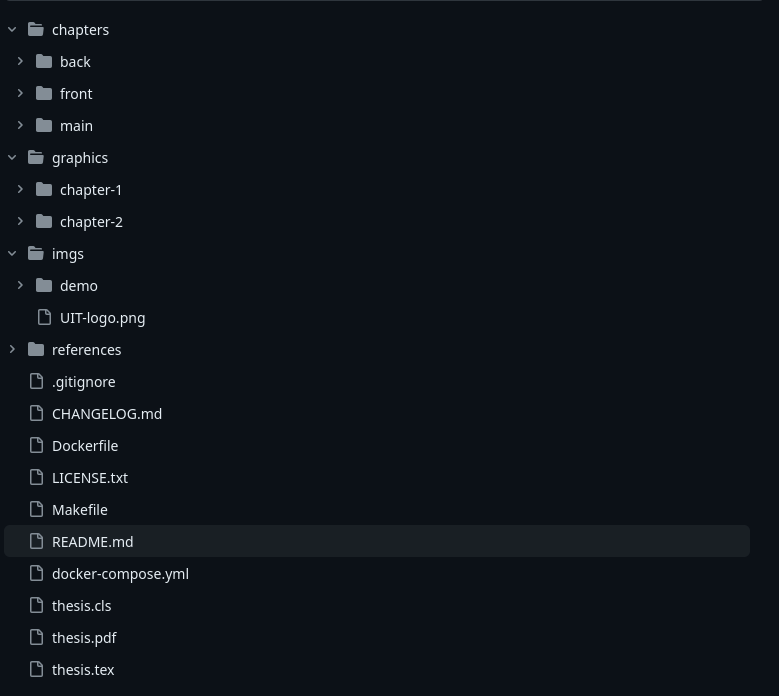
\includegraphics[scale=0.5]{chapter1/chap1-project-directory.png}
    \caption{Cấu trúc thư mục của dự án}
    \label{fig:chap1-project-directory}
\end{figure}

Thư mục \textbf{\textit{front}} tương ứng với các trang thông tin hội đồng chấm tốt nghiệp, lời cảm ơn, danh mục từ viết tắt... Thư mục \textbf{\textit{main}} chứa các chương của báo cáo. Báo cáo đánh số thứ tự riêng cho phần \textit{\textbf{front}}, trong khi phần các chương chính và phần phụ lục được đánh số giống nhau. Báo cáo đánh số trang bắt đầu từ trang tóm tắt, chữ số Ả-rập, bắt đầu bằng 1.

Thư mục \textbf{\textit{graphics}} chứa hình ảnh được chèn vào báo cáo. Tương ứng với mỗi chương sẽ có 1 thư mục hình ảnh của chương đó.

Thư mục \textbf{\textit{imgs}} là thư mục chứa hình ảnh của dự án, nó bao gồm các logo, watermark hoặc hình ảnh phục vụ cho document trên github. Hình chèn vào báo cáo không được lưu trong thư mục này.

Thư mục \textbf{\textit{references}} chứa các file chỉ mục tài liệu tham khảo. Tương tự như mỗi chapter một file .tex, nó cũng có riêng một file .bib để chỉ rõ các tài liệu tham khảo nào được sử dụng trong chuong nào.

File \textbf{\textit{thesis.cls}} là file quy định các câu lệnh, mức chỉ mục đánh số hình ảnh, bảng biểu, phần, chương. Quy định header và footer, trang  bìa.... Chi tiết xem trong file. Hãy chắc chắn rằng bạn hiểu rõ tất cả nếu muốn thay đổi gì trong file này.

File \textbf{\textit{thesis.tex}} là file quy định cấu trúc báo cáo, chương nào trước, chương nào sau, quy định thư mục hình ảnh chèn trong báo cáo. Nó quy định thông tin người báo cáo thông qua các câu lệnh được quy định trong file .cls. 

\section{Thay đổi các biến khi sử dụng}

Hai bìa của luận văn được tự động tạo bởi latex. Vì vậy, có các biến được quy định để đảm nhiệm nó. Các biến cần thay đổi được đặt tại thư mục gốc, tập tin \textit{thesis.tex}, được thể hiện trong hình \ref{fig:chap1-information-variable}.

\begin{figure}
    \centering
    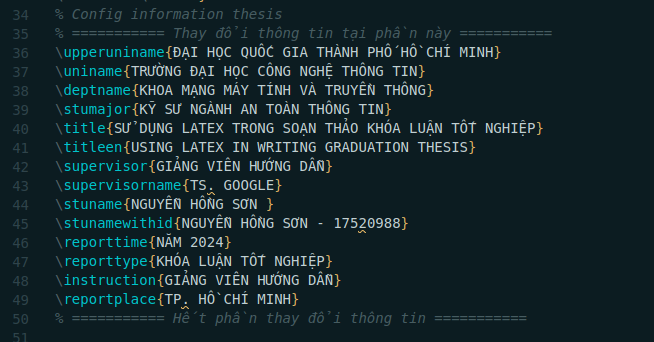
\includegraphics[scale=0.7]{chapter1/chap1-information-variable.png}
    \caption{Phần thay đổi thông tin trang bìa}
    \label{fig:chap1-information-variable}
\end{figure}

Các phần tiếp theo, quy định các nội dung được thêm vào báo cáo chính. Nếu một tập tin xuất hiện trong thư mục chapters nhưng không được khai báo bằng lệnh \textit{include} thì cũng không xuất hiện trong báo cáo. Vậy nên các chương mới bắt buộc phải được khai báo trong \textit{thesis.tex}. Các phần tài liêu tham khảo cũng được hiểu tương tự.


\chapter{Phương pháp chèn hình ảnh}
\label{chap:chap2-figures}
Trong một luận văn hay báo cáo, các hình ảnh được sử dụng rất nhiều. Việc chèn hình ảnh tuy đơn giản nhưng cần sử dụng nhiều kỹ thuật. Chương này trình bày các cách chèn hình ảnh từ đơn giản tới phức tạp.

\section{Chèn hình ảnh đơn điệu}

Chèn hình ảnh đơn điệu nghĩa là chỉ chèn một hình ảnh cơ bản, có cú pháp latex như sau:

\begin{lstlisting}[language={[LaTeX]TeX}, caption={Chèn một hình ảnh vào báo cáo}, label={lst:figure}]
\begin{figure}
    \centering
    \includegraphics[scale=0.7]{chapter1/figure-url.png}
    \caption{Caption of figure}
    \label{fig:figure-label}
\end{figure}
\end{lstlisting}

Hình ảnh từ đường dẫn \textit{chapter1/figure-url.png} sẽ được chèn vào báo cáo với kích thuớc bằng \textit{scale=0.7}. Hình ảnh sẽ có chú tích là \textit{Caption of figure}, nhãn \textit{fig:figure-label} sẽ được sử dụng để chỉ mục tới hình ảnh.

\section{Chèn nhiều hình ảnh trong một hình ảnh}

Trong tình huống cần chèn nhiều hình ảnh nhưng bản thân những hình ảnh này có tương quan đến nhau. Ví dụ tại hình \ref{fig:chap2-subfigure-example}, hai hình ảnh thể hiện trạng thái của đối tượng trong các ngữ cảnh khác nhau. Đây là lúc chúng ta cần sử dụng hình ảnh con.

Một hinh ảnh với nhiều hình ảnh con được chèn vào báo cáo như sau \cite{ShantoLatex}:

\begin{lstlisting}[language={[LaTeX]TeX}, caption={Chèn nhiều hình ảnh con trong một hình ảnh}, label={lst:example-subfigure}]
\begin{figure}
    \begin{subfigure}{0.5\textwidth}
        \centering
        \includegraphics[scale=0.3]{chapter1/subfigure-example.png}
        \caption{Caption of figure 1}
        \label{fig:sub-figure-url-1}
    \end{subfigure}
    \begin{subfigure}{0.5\textwidth}
        \centering
        \includegraphics[scale=0.3]{chapter1/subfigure-example.png}
        \caption{Caption of figure 2}
        \label{fig:sub-figure-url-2}
    \end{subfigure}
    \caption{Caption of figure}
    \label{fig:example-subfigure}
\end{figure}
      
\end{lstlisting}

Một lưu ý khi sử dụng hình ảnh con thì các hình ảnh nên có kích thước giống nhau để đạt độ hiệu quả cao nhất.

\begin{figure}
    \begin{subfigure}{0.5\textwidth}
        \centering
        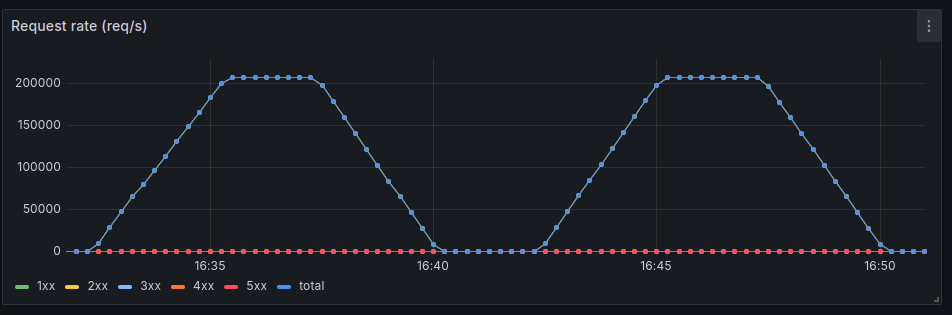
\includegraphics[scale=0.3]{chapter2/chap2-subfigure-example.png}
        \caption{Caption of figure 1}
        \label{fig:chap2-subfigure-example-1}
    \end{subfigure}%
    \begin{subfigure}{0.5\textwidth}
        \centering
        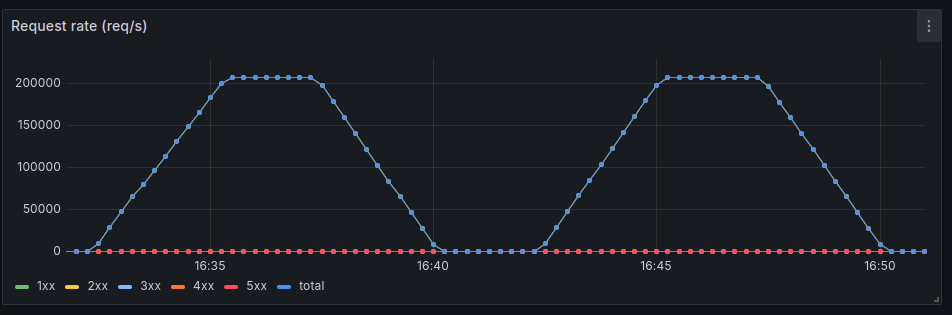
\includegraphics[scale=0.3]{chapter2/chap2-subfigure-example.png}
        \caption{Caption of figure 2}
        \label{fig:chap2-subfigure-example-2}
    \end{subfigure}
    \caption{Mô tả chèn hình ảnh con trong một hình ảnh lớn}
    \label{fig:chap2-subfigure-example}
\end{figure}

\section{Chèn hình ảnh với ghi chú ở bên cạnh}

Chèn hình ảnh toàn trang thì tương đối dễ, ta chỉ việc chèn hình đó với độ thu phóng phù hợp. Phần này trình bày việc chèn các hình ảnh toàn trang và có ghi chú nằm ở vị trí khác so với bình thường.

Hình \ref{fig:img-caption-rotate} minh họa hình ảnh và ghi chú của nó được xoay một góc $90^{\circ}$. Đoạn mã \ref{lst:figure-with-caption-rotate} giúp ta làm được điều này.

\begin{figure}
    \begin{minipage}[c]{0.8\textwidth}
      \centering
      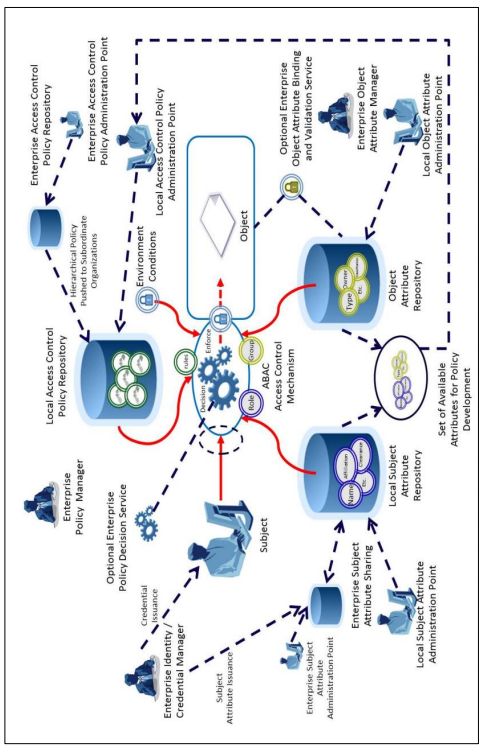
\includegraphics[width=\textwidth]{chapter2/chap2-rotate-figure-example.png} 
    \end{minipage}
    \begin{minipage}[c]{0.1\textwidth}
      \begin{adjustbox}{angle=90,center}
        \begin{minipage}[c]{\textheight}
          \caption{Minh họa chèn hình ảnh với caption xoay $90^{\circ}$}
          \label{fig:img-caption-rotate}
        \end{minipage}
      \end{adjustbox}
    \end{minipage}
\end{figure}

\begin{lstlisting}[language={[LaTeX]TeX}, caption={Chèn hình ảnh với caption xoay $90^{\circ}$}, label={lst:figure-with-caption-rotate}]
\begin{figure}
    \begin{minipage}[c]{0.8\textwidth}
        \centering
        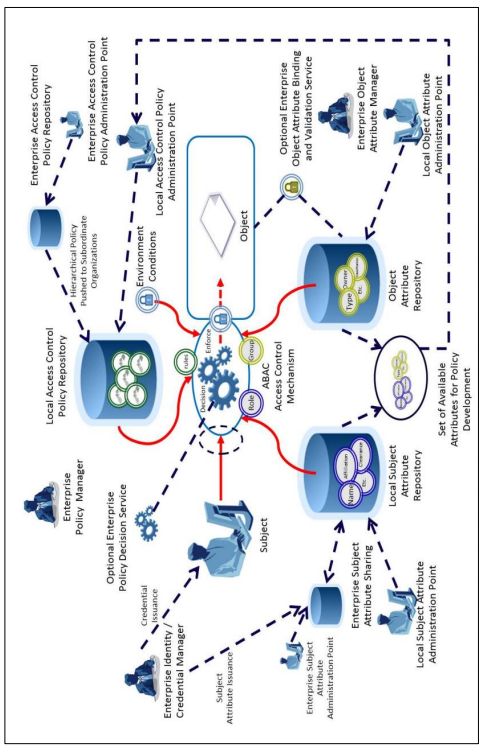
\includegraphics[width=\textwidth]{chapter2/chap2-rotate-figure-example.png} 
    \end{minipage}
    \begin{minipage}[c]{0.1\textwidth}
        \begin{adjustbox}{angle=90,center}
        \begin{minipage}[c]{\textheight}
            \caption{Figure caption}
            \label{fig:img-caption-rotate}
        \end{minipage}
        \end{adjustbox}
    \end{minipage}
\end{figure}
\end{lstlisting}

Trong một số trường hợp, ta chỉ cần caption ở một bên hình ảnh chứ không xoay như hình \ref{fig:img-just-caption-side}, ta chỉ cần thực hiện như đoạn mã \ref{lst:figure-just-caption-side}.

\begin{figure}
    \begin{minipage}[c]{0.7\textwidth}
      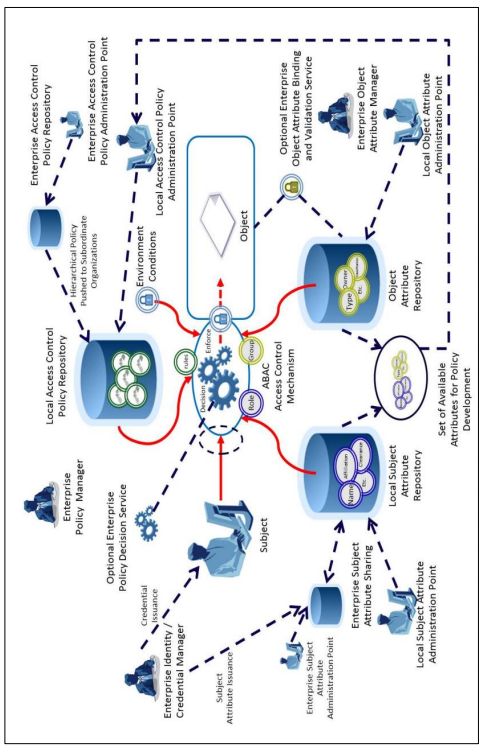
\includegraphics[width=\textwidth]{chapter2/chap2-rotate-figure-example.png}
    \end{minipage}\hfill
    \begin{minipage}[c]{0.2\textwidth}
      \caption{
        Figure caption
      } \label{fig:img-just-caption-side}
    \end{minipage}
\end{figure}

\begin{lstlisting}[language={[LaTeX]TeX}, caption={Chèn hình ảnh với caption ở bên phải $90^{\circ}$}, label={lst:figure-just-caption-side}]
\begin{figure}
    \begin{minipage}[c]{0.7\textwidth}
        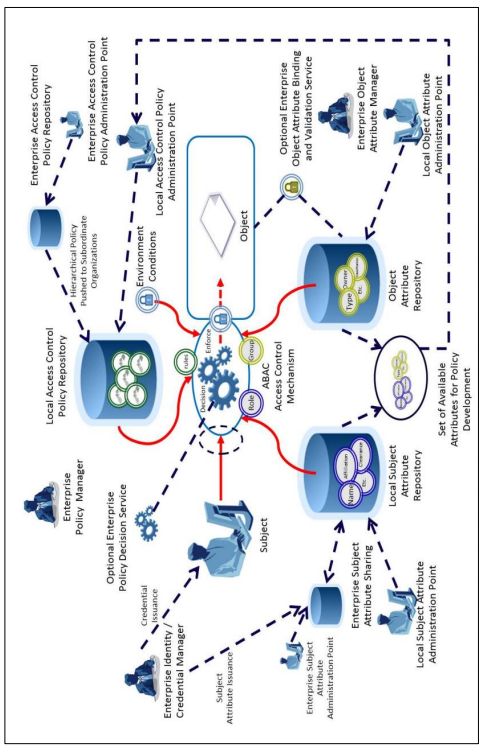
\includegraphics[width=\textwidth]{chapter2/chap2-rotate-figure-example.png}
    \end{minipage}\hfill
    \begin{minipage}[c]{0.2\textwidth}
        \caption{
            Figure caption
        } \label{fig:img-just-caption-side}
    \end{minipage}
\end{figure}
\end{lstlisting}
\chapter{Phương pháp chèn bảng}
\label{chap:chap3-table}

Chương này trình bày một số kỹ thuật chèn bảng với các cột, dòng merge nhiều ô. Các cách format bảng cơ bản không trình bày. Trong quá trình sử dụng, có thể cập nhật các chỉ dẫn rõ ràng cho từng câu lệnh nghĩa là gì trong một bảng.




% Appendix chapter in thesis
\appendix
\chapter{Hướng dẫn soạn phụ lục}

% Print references
\printbibliography[heading=bibintoc, title = {Tài liệu tham khảo}]
\end{document}
